\documentclass[11pt, a4paper, twoside]{article}
\usepackage{graphicx}
\usepackage{amsmath}
\usepackage[margin=0.8in]{geometry}
\usepackage{listings}
\usepackage{float}
\usepackage{fancyhdr}
\usepackage{indentfirst}
\usepackage[inline]{enumitem}
\usepackage{tabularx}
\usepackage{xcolor}
\usepackage{array}
\usepackage{minted}
\usemintedstyle{vs}
\usepackage[belowskip=0pt,aboveskip=0pt,font=small,labelfont=small]{caption}
\captionsetup{width=\linewidth}
\setlength\intextsep{0pt}
\graphicspath{{Plots/}}
\setlist[itemize]{noitemsep, topsep=0pt}
\fancyhead[RO,LE]{EE2703: Assignment 7}
\fancyhead[LO,RE]{Akilesh Kannan}
\cfoot{\thepage}

\title{EE2703: Assignment 7}
\author{Akilesh Kannan (EE18B122)}
\date{\today}

\pagestyle{fancy}

\begin{document}
\maketitle

\section{Introduction}
The aim of this assignment is to analyse circuits using the Symbolic algebra capabilities of \texttt{Sympy}.

\section{Low-Pass Filter}
    In this section, we analyse the following circuit:
    \begin{figure}[H]
        \centering
        \includegraphics[scale=0.25]{circuits/ckt1.png}
        \caption{Op-Amp based Low-Pass Filter}
        \label{fig:ckt1}
    \end{figure}
    Writing KCL equations (in $s$-domain) of the nodes marked on the figure, we get the following matrix:
    \begin{equation}
        \begin{pmatrix}
            0&0&1&\frac{-1}{G}\\
            \frac{-1}{1+sR_2C_2}&1&0&0\\
            0&-G&G&1\\
            -\frac{1}{R_1}-\frac{1}{R_2}-sC_1&\frac{1}{R_2}&0&sC_1\\
        \end{pmatrix}
        \begin{pmatrix}
            V_1(s)\\
            V_p(s)\\
            V_m(s)\\
            V_o(s)\\
        \end{pmatrix}
        =
        \begin{pmatrix}
            0\\
            0\\
            0\\
            \frac{V_i(s)}{R_1}\\
        \end{pmatrix}
    \end{equation}
    \texttt{Sympy} allows us to create matrices with symbolic entries, and also perform mathematical operations on them, as if they were \texttt{numpy} arrays. In the above circuit, the values of $R_1$, $R_2$, $C_1$, $C_2$ are $10k\Omega$, $10k\Omega$, $10$pF, $10$pF respectively.\\
    
    Solving for $V_o(s)$, (with the above given values) we get:
    \begin{equation}
        V_o(s) = \frac{-0.0001586\cdot V_i(s)}{2\times10^{-14}s^2 + 4.414\times10^{-9}s + 0.0002}
        \label{eq2}
    \end{equation}
    
    From \eqref{eq2}, we get the step response of the circuit as:
    \begin{equation}
        V_o(s) = \frac{-0.0001586\cdot \frac{1}{s}}{2\times10^{-14}s^2 + 4.414\times10^{-9}s + 0.0002}
    \end{equation}
    
    \texttt{Sympy} allows us to convert a symbolic expression into functions that are compatible with other packages like \texttt{numpy}, \texttt{scipy} etc. This can be accomplished by converting the expression into a \textit{lambda}\footnote{Lambda functions are, in a nutshell, \textit{one-time use} functions. They are short-lived functions, very useful for quick manipulations, especially inside other functions.} function. For this purpose, \texttt{sympy} has a method called \textit{lambdify}, which takes in as arguments, the symbols in the expression (which are to be treated as variables), the expression itself, and also the package with which the resulting function has to be compatible with.
    
    However, since we are required to use the \texttt{scipy.signal} toolbox, we have to convert the above the symbolic expression to a format with which we can easily create a \texttt{signal.lti} object. For that, we extract the coefficients of the numerator and denominator polynomials of $V_o(s)$ and create a \texttt{signal.lti} object using the same. The below piece of code accomplishes this:
    \inputminted[breaklines, linenos]{python}{code/sympyToLTI.py}
    
    Now, we can easily create a \texttt{signal.lti} object with the coefficients we got, and use \texttt{signal.bode} to obtain the Bode magnitude and phase plots, which are shown below.
    \begin{figure}[H]
        \centering
        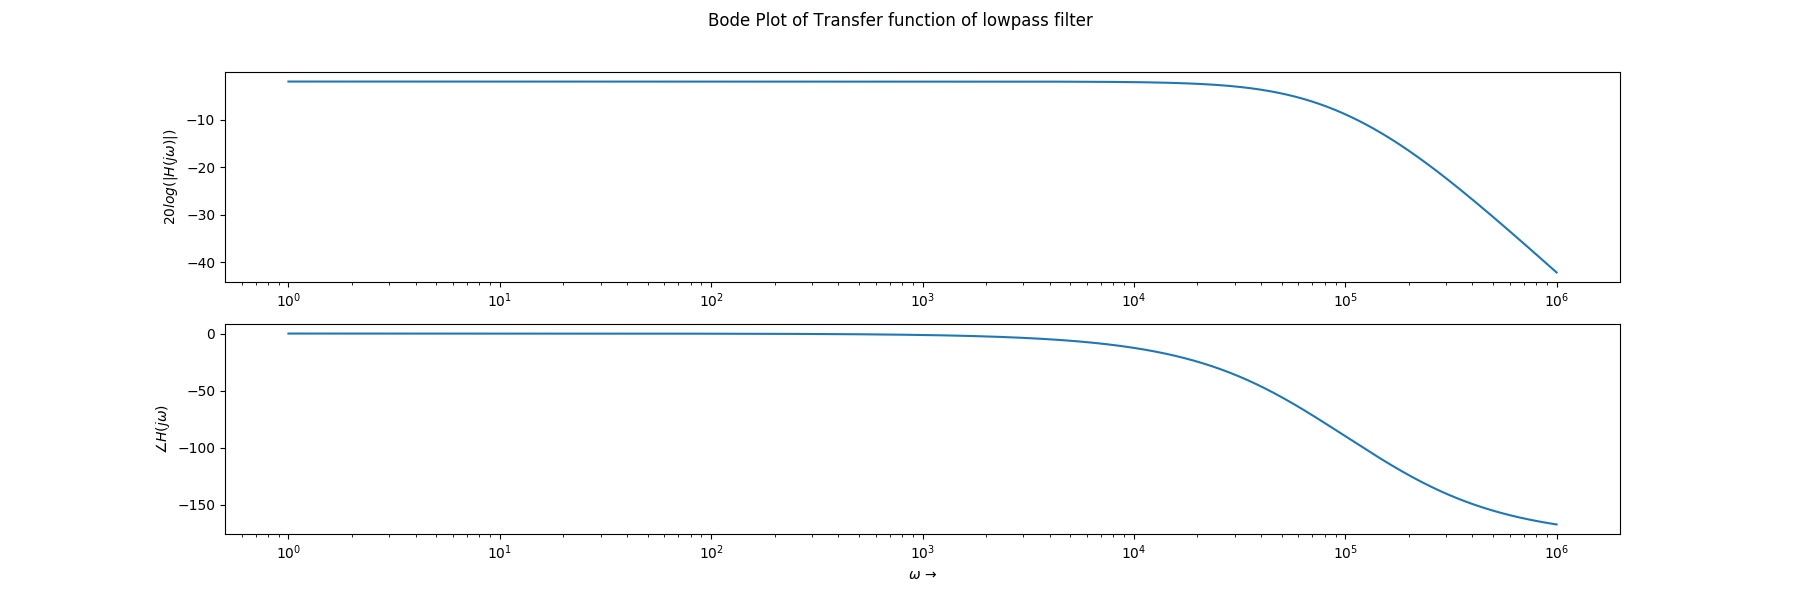
\includegraphics[scale=0.4]{plots/Fig 1.png}
        \caption{Bode Magnitude and Phase plots of step response of LPF}
        \label{fig:Fig2}
    \end{figure}
    
    To see the step response of the system, we can use \texttt{signal.step}. The step response of the system is shown below.
    \begin{figure}[H]
        \centering
        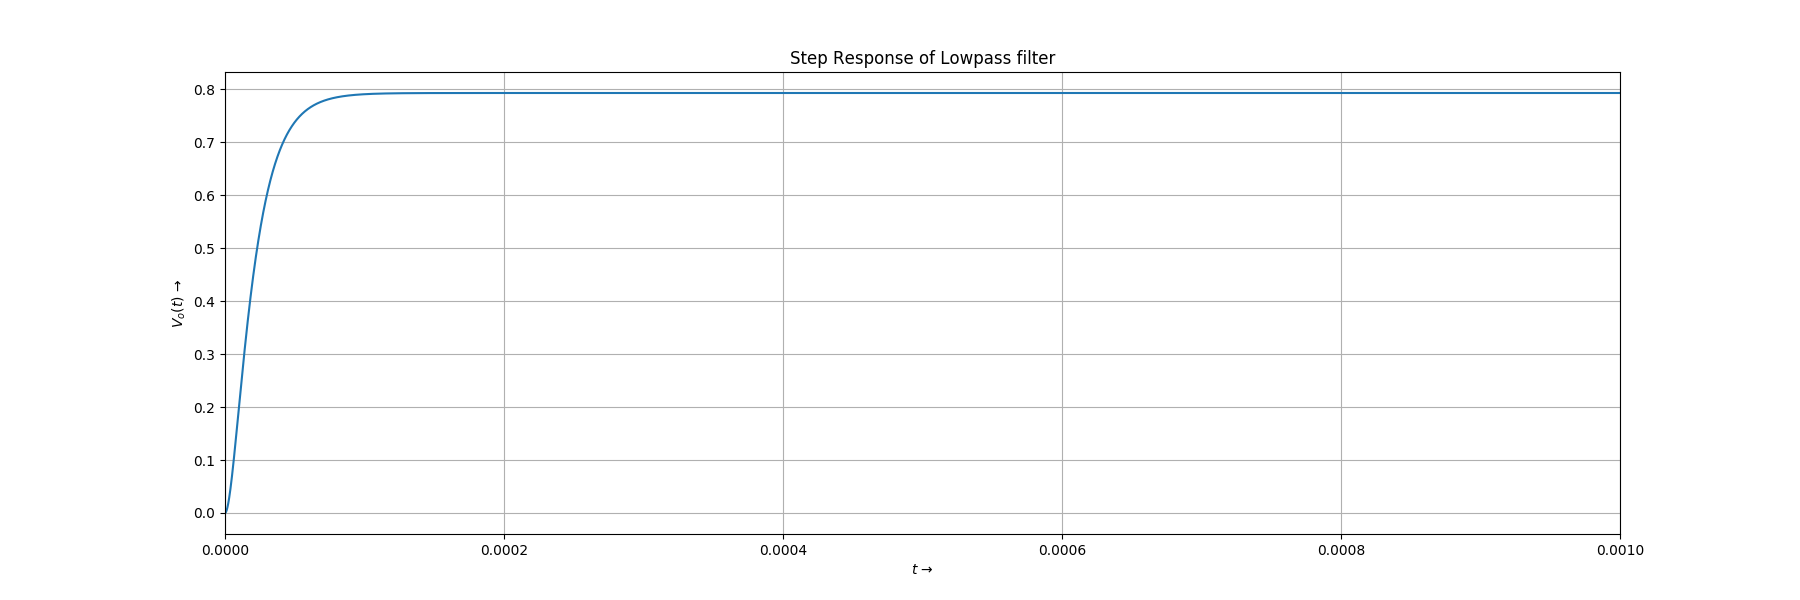
\includegraphics[scale=0.4]{plots/Fig 2.png}
        \caption{Step response of LPF}
        \label{fig:Fig3}
    \end{figure}
    
    Now, we shall see that the circuit is indeed a low-pass filter by plotting the output for a mixed-frequency input, which has both high frequency and low frequency components.
    
    We shall give the following input to the filter:
    \begin{equation}
        v_i(t) = (sin(2\pi\times 10^3t)+cos(2\pi\times 10^6t))u(t)
        \label{eq4}
    \end{equation}
    
    We shall use \texttt{signal.lsim} to calculate the time-domain response of the system.
    
    \begin{figure}[H]
        \centering
        \setlength\tabcolsep{1pt}
        \begin{tabular}{cc}
            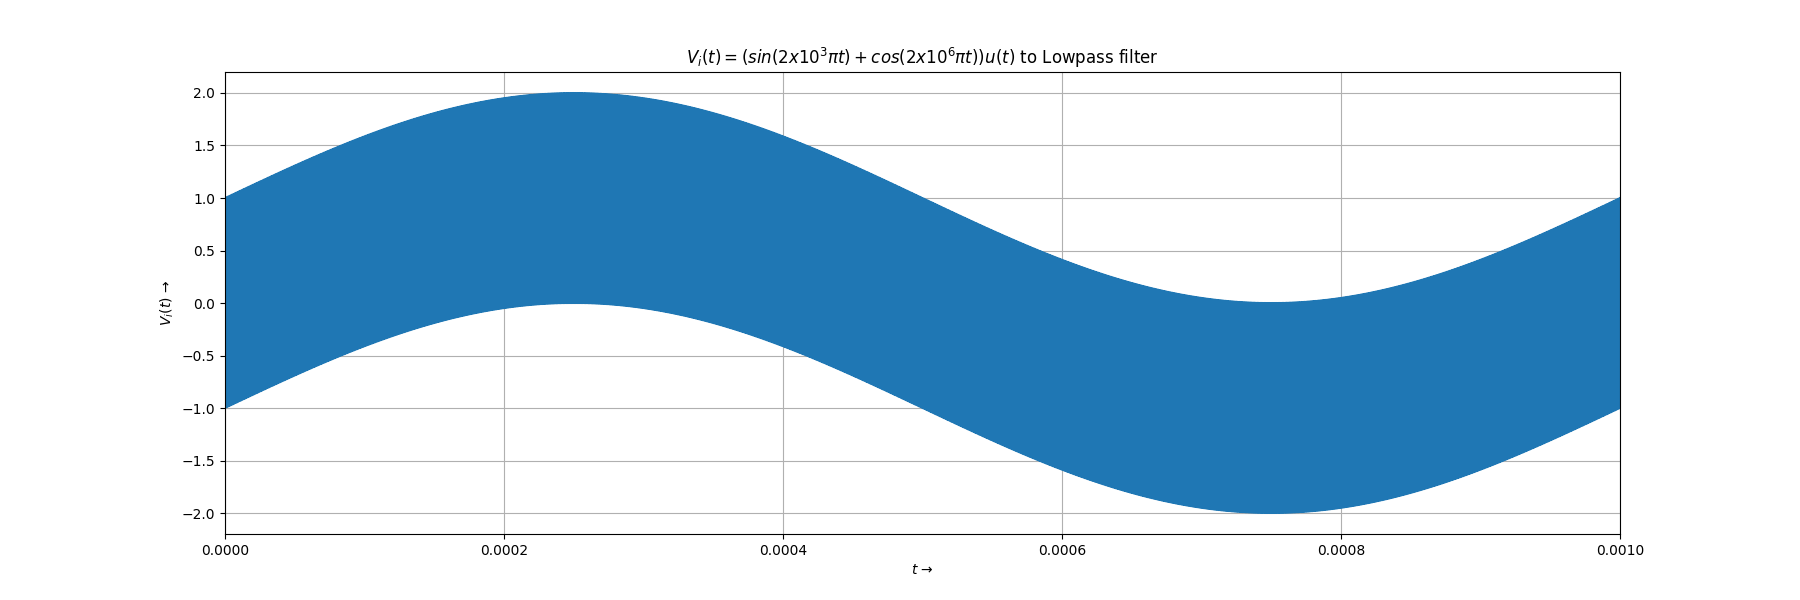
\includegraphics[width=0.55\textwidth]{plots/Fig 3.png} &
            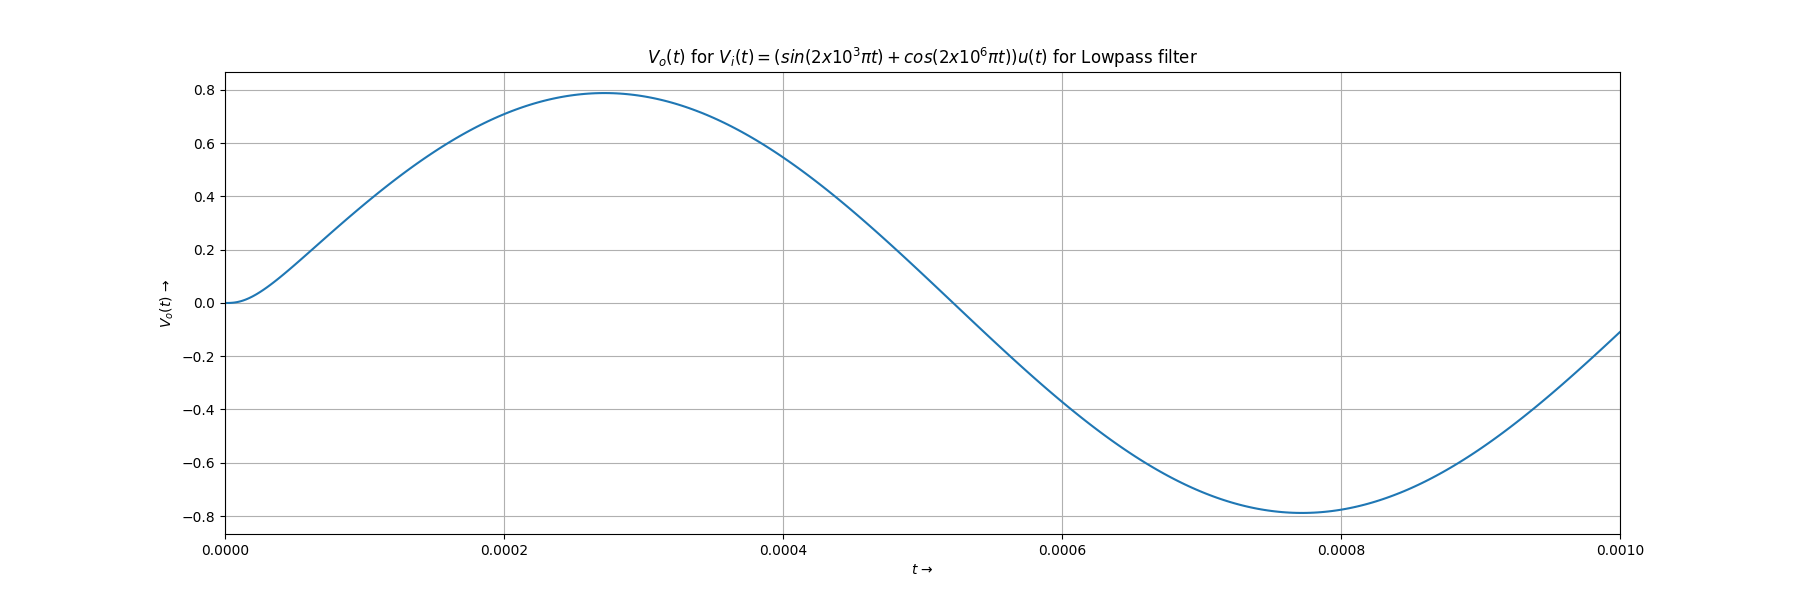
\includegraphics[width=0.55\textwidth]{plots/Fig 4.png}\\
        \end{tabular}
        \caption{\textit{Left}: Mixed frequency input\\\textit{Right}: Filtered Output}
    \end{figure}
    
    We can easily see that the output contains only the low frequency component of the input ($1\ KHz$ sinusoid). Thus, the circuit is a low-pass filter. It's cut-off frequency for the values of $R_1$, $R_2$, $C_1$, $C_2$ used is $\frac{1}{2\pi}\ MHz$.
    
\section{High-Pass Filter}

We shall now look at a slightly modified version of the above circuit.
\begin{figure}[H]
    \centering
    \includegraphics[scale=0.25]{circuits/ckt2.png}
    \caption{Op-amp based High-Pass Filter}
    \label{fig:fig5}
\end{figure}

Performing a similar procedure like before, we get the KCL matrix as:
\begin{gather}
    \begin{pmatrix}
            0&0&1&\frac{-1}{G}\\
            \frac{sR_3C_2}{1+sR_3C_2}&0&-1&0\\
            0&-G&G&1\\
            -\frac{1}{R_1}-sC_2-sC_1&0&sC_2&\frac{1}{R_1}\\
        \end{pmatrix}
        \begin{pmatrix}
            V_1(s)\\
            V_p(s)\\
            V_m(s)\\
            V_o(s)\\
        \end{pmatrix}
        =
        \begin{pmatrix}
            0\\
            0\\
            0\\
            -sC_1V_i(s)\\
        \end{pmatrix}
\end{gather}

Solving it for $V_o(s)$, we get, 
\begin{equation}
    V_o(s) = \frac{1.586\times10^{-14}s^2\cdot V_i(s)}{2\times10^{-14}s^2 + 4.414\times10^{-9}s + 0.0002}
\end{equation}
The Bode magnitude and phase plots of the transfer function as:
\begin{figure}[H]
    \centering
    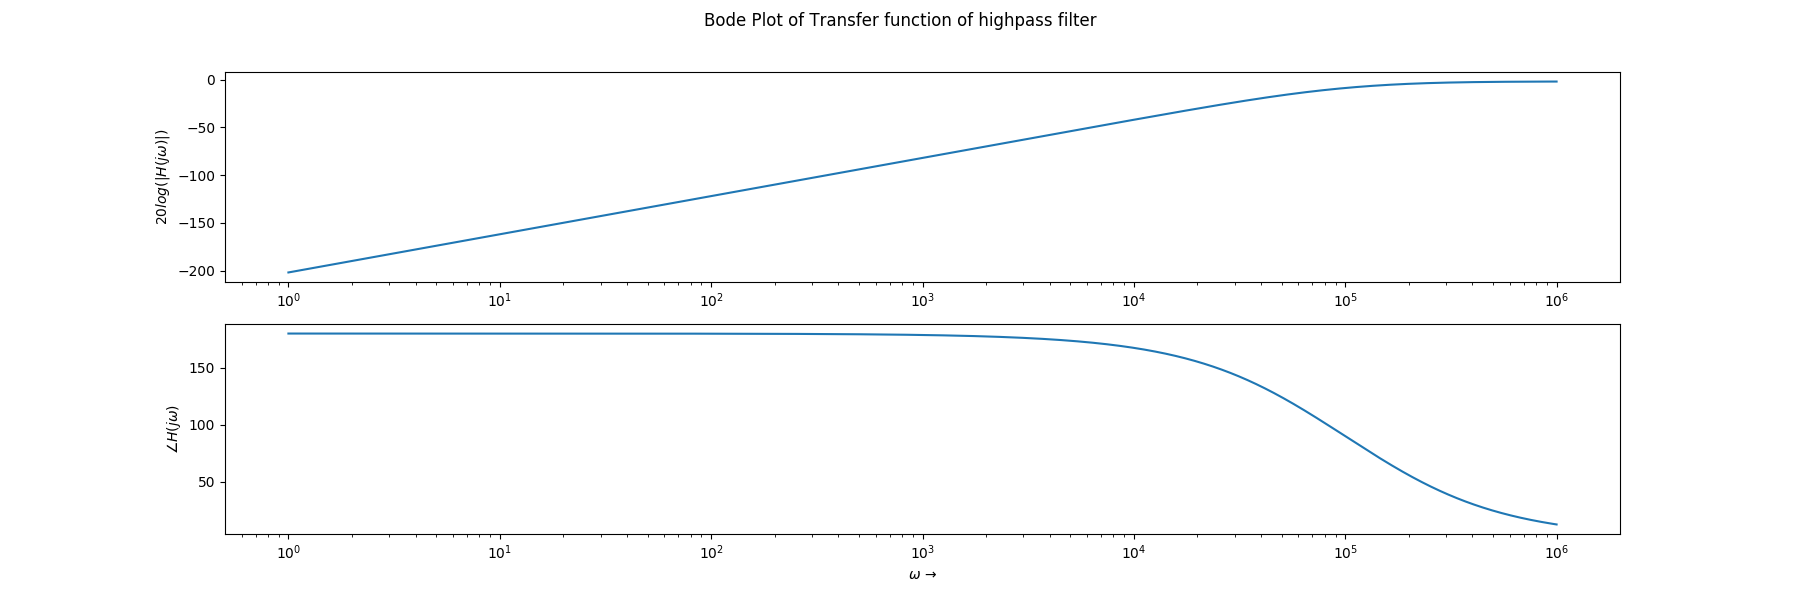
\includegraphics[scale=0.4]{plots/Fig 5.png}
    \caption{Bode Magnitude and Phase plots of step response of HPF}
    \label{fig:Fig6}
\end{figure}

The step response of the circuit was obtained as:

\begin{figure}[H]
    \centering
    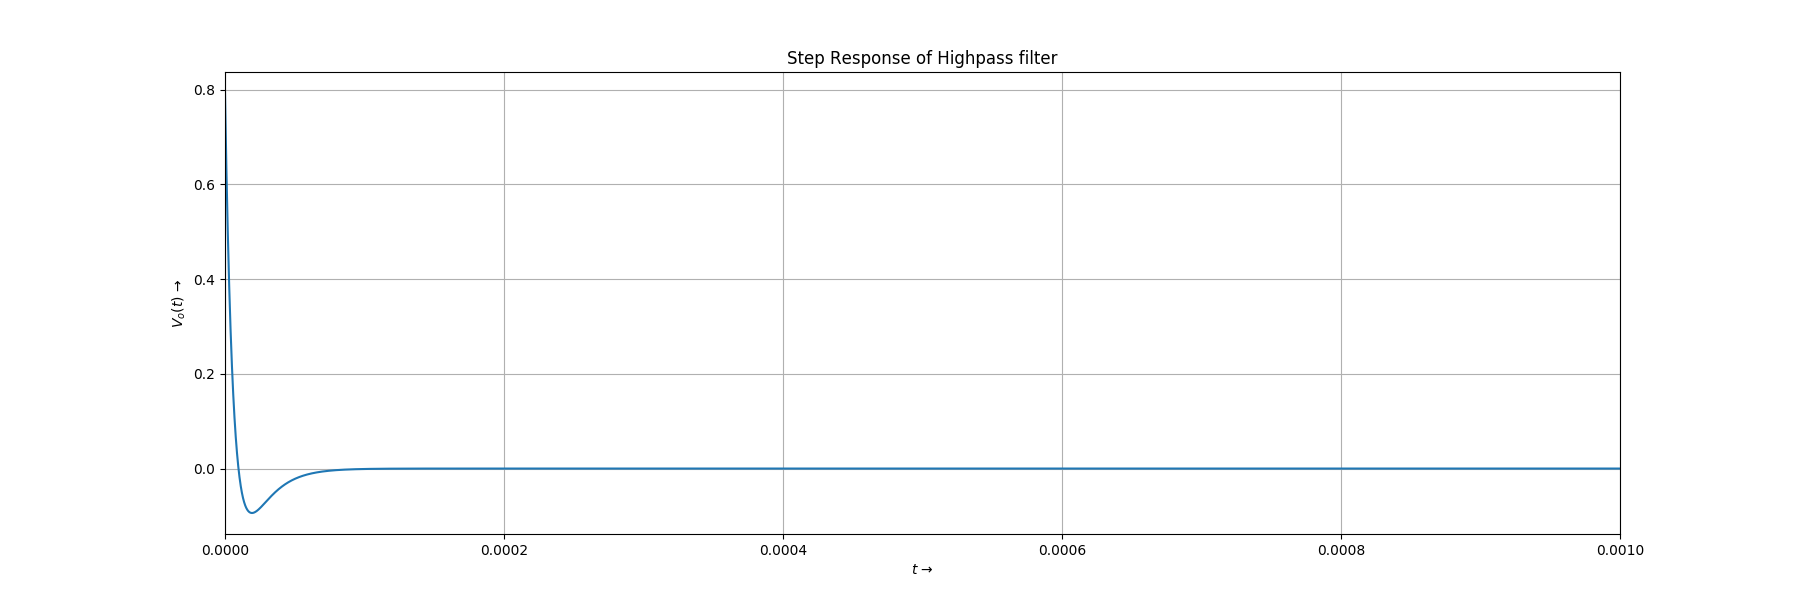
\includegraphics[scale=0.4]{plots/Fig 10.png}
    \caption{Step Response of HPF}
    \label{fig:Fig7}
\end{figure}

The response to the mixed frequency input in Eq \eqref{eq4} is:

\begin{figure}[H]
    \centering
    \setlength\tabcolsep{1pt}
    \begin{tabular}{cc}
        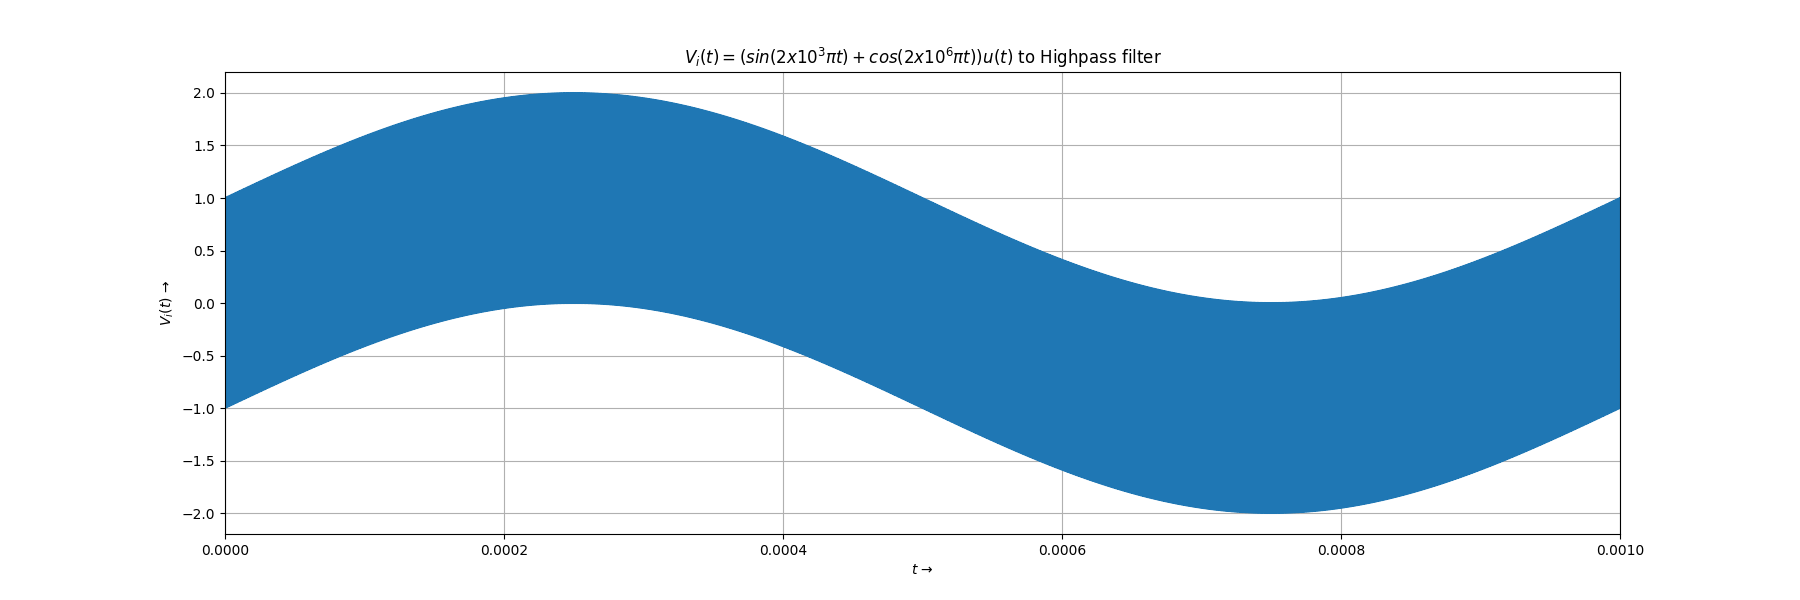
\includegraphics[width=0.55\textwidth]{plots/Fig 6.png} &
        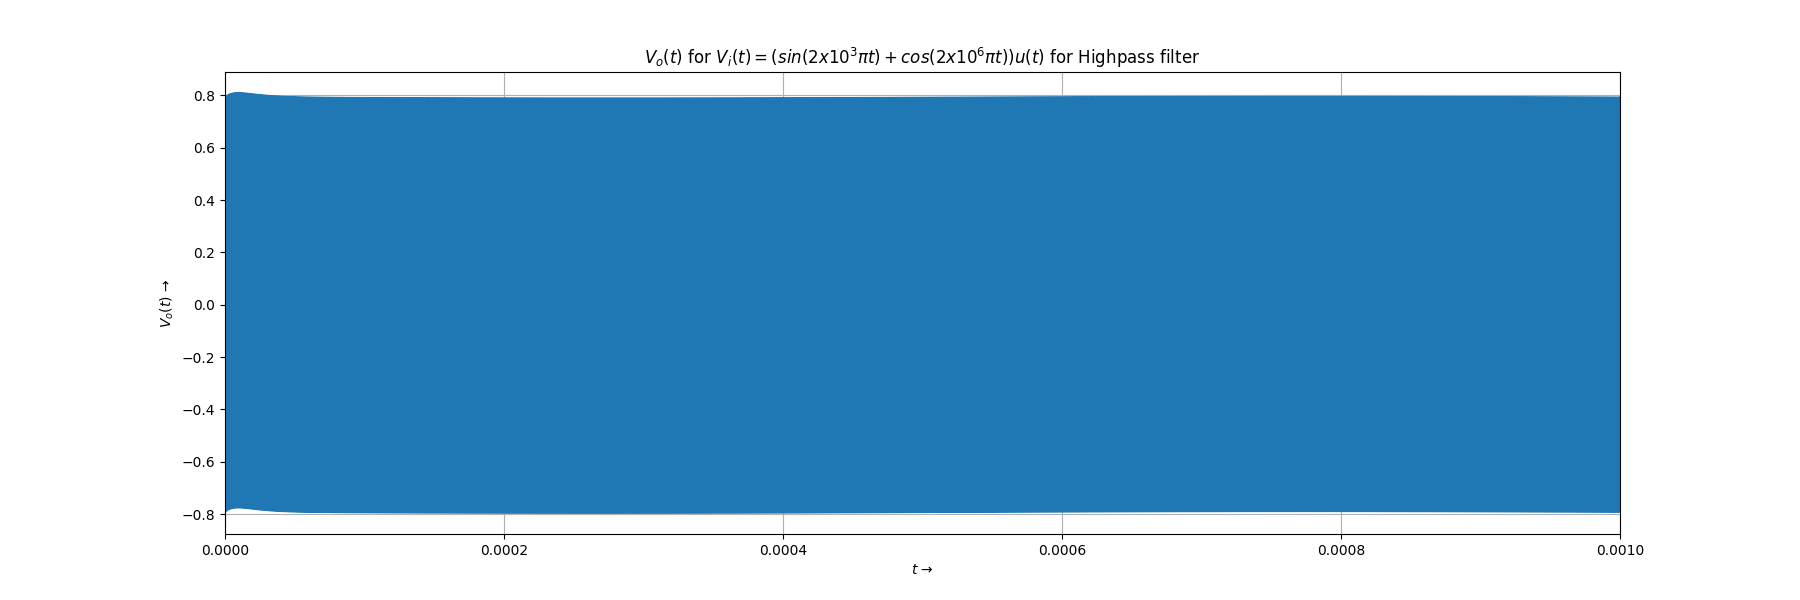
\includegraphics[width=0.55\textwidth]{plots/Fig 7.png}\\
    \end{tabular}
    \caption{\textit{Left}: Mixed frequency input\\\textit{Right}: Filtered Output}
\end{figure}
    
We shall look at the response of the system to a damped sinusoid. We shall consider two of them - one of high frequency (0.1 MHz) and the other of low frequency (1 Hz).

\begin{figure}[H]
    \centering
    \setlength\tabcolsep{1pt}
    \begin{tabular}{cc}
        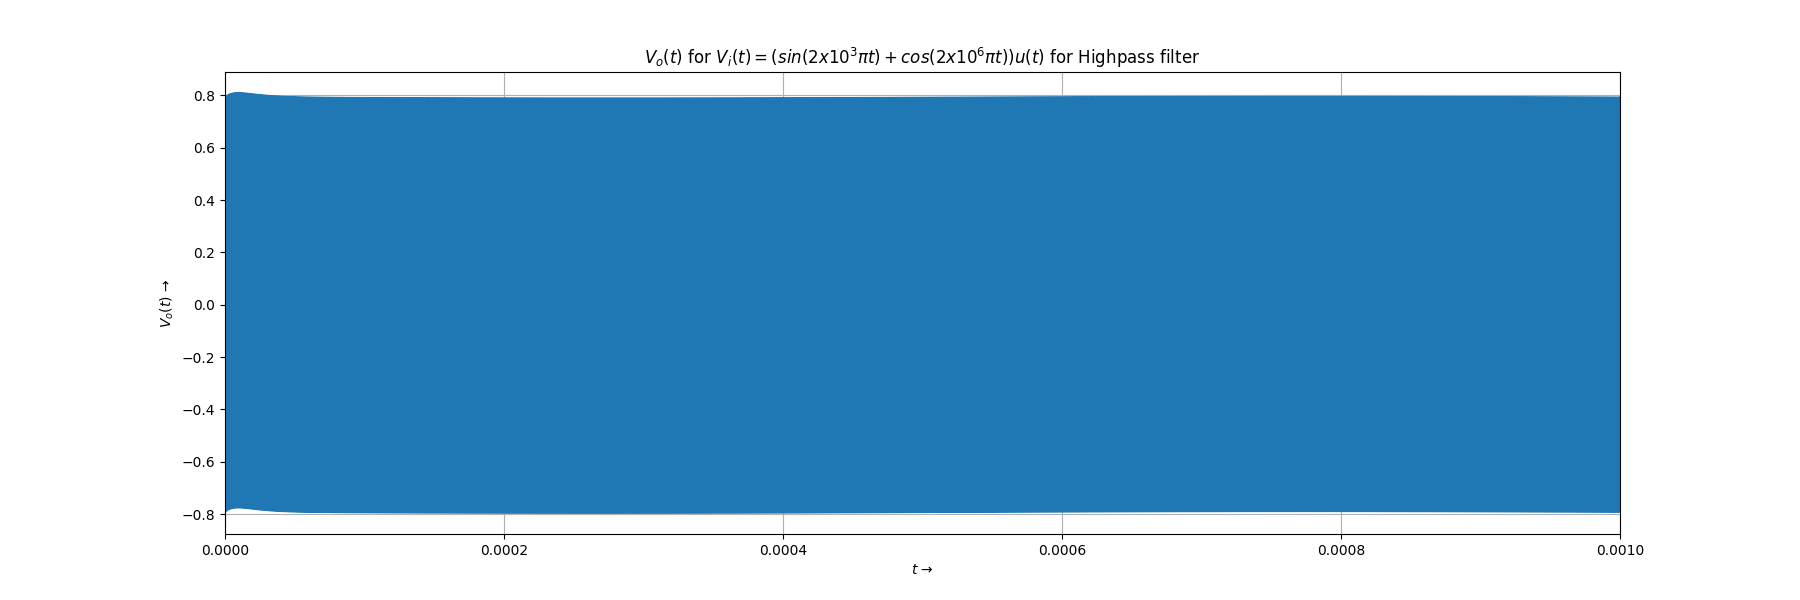
\includegraphics[width=0.55\textwidth]{plots/Fig 8.png} &
        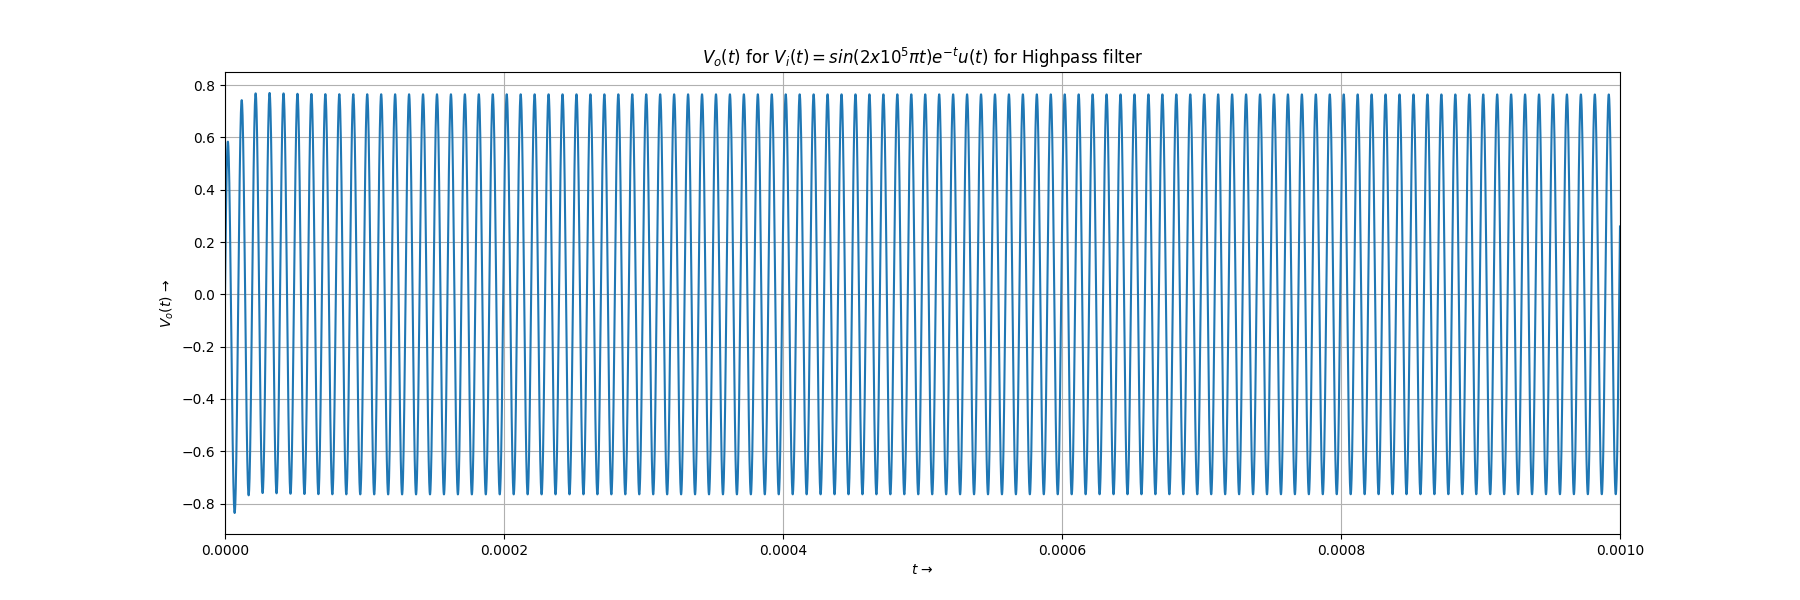
\includegraphics[width=0.55\textwidth]{plots/Fig 9.png}\\
    \end{tabular}
    \caption{\textit{Left}: Low frequency input\\\textit{Right}:High frequency input}
\end{figure}

We get that the output of the filter if the input is a low frequency damped sinusoid is 0, except for initial transients. This is expected due to the inherent nature of the circuit to act as a high-pass filter. This is why we can see that it allows the high-frequency input to pass through.

\section{Conclusion}
\texttt{Sympy} provides a convenient way to analyse LTI systems using their Laplace transforms.  The toolbox was used to study the behaviour of a low pass filter,implemented using an op-amp of gain G. For a mixed frequency sinusoid as input,  it  was  found  that  the  filter  suppressed  the  high  frequencies  while allowing  the  low  frequency  components.   Similarly,  a  high  pass  filter  was implemented using an op-amp with the same gain.  The magnitude response of the filter was plotted and its output was analysed for damped sinusoids.The step response of the filter was found to have a non-zero peak at $t= 0$ ,due to the sudden change in the input voltage.
\end{document}
